% -*- Mode:TeX -*-

%% IMPORTANT: The official thesis specifications are available at:
%%
%%            Please verify your thesis' formatting and copyright
%%            assignment before submission.  If you notice any
%%            discrepancies between these templates and the
%%            MIT Libraries' specs, please let us know
%%            by e-mailing thesis@mit.edu

%% The documentclass options along with the pagestyle can be used to generate
%% a technical report, a draft copy, or a regular thesis.  You may need to
%% re-specify the pagestyle after you \include  cover.tex.  For more
%% information, see the first few lines of mitthesis.cls. 

%\documentclass[12pt,vi,twoside]{mitthesis}
%%
%%  If you want your thesis copyright to you instead of MIT, use the
%%  ``vi'' option, as above.
%%
%\documentclass[12pt,twoside,leftblank]{mitthesis}
%%
%% If you want blank pages before new chapters to be labelled ``This
%% Page Intentionally Left Blank'', use the ``leftblank'' option, as
%% above. 
% Add all your packages here


\documentclass[12pt,twoside]{mitthesis}
\usepackage{enumerate}
\usepackage{graphicx} 
\def\spanishoptions{mexico}
\usepackage[spanish]{babel}
%\usepackage[T1]{fontenc}
%\usepackage[utf8]{inputenc}
\usepackage{amsmath} 
\usepackage{lgrind}
\usepackage{listings}
\usepackage{color}
\usepackage{float}
\usepackage{placeins}


\usepackage{ifxetex}

\ifxetex
  \usepackage{fontspec}
\else
  \usepackage[T1]{fontenc}
  \usepackage[utf8]{inputenc}
  \usepackage{lmodern}
\fi

\usepackage{caption}
%\DeclareCaptionFormat{myformat}{#1#2#3}
\newlength\myindention
\DeclareCaptionFormat{myformat}%
{#1#2#3 \hspace*{\myindention}}
\captionsetup{format=myformat}
\captionsetup[lstlisting]{position=bottom,format=myformat}
\renewcommand{\lstlistingname}{Algoritmo}

\usepackage{fancyhdr}
\pagestyle{fancy}

\fancyhead{}
\fancyfoot{}

\fancyhead[RO,RE]{\fontsize{10}{12} \selectfont \thepage}
\fancyhead[LO]{\fontsize{10}{12} \selectfont \leftmark}
\fancyhead[LE]{\fontsize{10}{12} \selectfont \leftmark}

\renewcommand{\headrulewidth}{0.0pt}
\renewcommand{\footrulewidth}{0.0pt}

\addto\captionsspanish{%
  \renewcommand{\appendixname}%
    {Anexos}%
}


%\usepackage{fontspec}
\setmainfont{Times New Roman}
%\setmainfont{Arial}


%\usepackage[T1,T2A]{fontenc}
%\usepackage[latin1]{inputenc}
%\usepackage[spanish]{babel}

%\selectlanguage{spanish}

%\pagestyle{plain}
 
%% This bit allows you to either specify only the files which you wish to
%% process, or `all' to process all files which you \include.
%% Krishna Sethuraman (1990).

% \typein [\files]{Enter file names to process, (chap1,chap2 ...), or
%  `all' to process all files:}
\def\all{all}
% \ifx\files\all \typeout{Including all files.} \else \typeout{Including only \files.} \includeonly{\files} \fi

\begin{document}

% -*-latex-*-
% 
% For questions, comments, concerns or complaints:
% thesis@mit.edu
% 
%
% $Log: cover.tex,v $
% Revision 1.8  2008/05/13 15:02:15  jdreed
% Degree month is June, not May.  Added note about prevdegrees.
% Arthur Smith's title updated
%
% Revision 1.7  2001/02/08 18:53:16  boojum
% changed some \newpages to \cleardoublepages
%
% Revision 1.6  1999/10/21 14:49:31  boojum
% changed comment referring to documentstyle
%
% Revision 1.5  1999/10/21 14:39:04  boojum
% *** empty log message ***
%
% Revision 1.4  1997/04/18  17:54:10  othomas
% added page numbers on abstract and cover, and made 1 abstract
% page the default rather than 2.  (anne hunter tells me this
% is the new institute standard.)
%
% Revision 1.4  1997/04/18  17:54:10  othomas
% added page numbers on abstract and cover, and made 1 abstract
% page the default rather than 2.  (anne hunter tells me this
% is the new institute standard.)
%
% Revision 1.3  93/05/17  17:06:29  starflt
% Added acknowledgements section (suggested by tompalka)
% 
% Revision 1.2  92/04/22  13:13:13  epeisach
% Fixes for 1991 course 6 requirements
% Phrase "and to grant others the right to do so" has been added to 
% permission clause
% Second copy of abstract is not counted as separate pages so numbering works
% out
% 
% Revision 1.1  92/04/22  13:08:20  epeisach

% NOTE:
% These templates make an effort to conform to the MIT Thesis specifications,
% however the specifications can change.  We recommend that you verify the
% layout of your title page with your thesis advisor and/or the MIT 
% Libraries before printing your final copy.

\title{Análisis de Sentimientos usando Dinámica de Tecleo y Dinámica
  de Ratón para el Secuenciado de Ejercicios de Programación de Computadoras}

\author{Amaury Hernández Águila}
% If you wish to list your previous degrees on the cover page, use the 
% previous degrees command:
%       \prevdegrees{A.A., Harvard University (1985)}
% You can use the \\ command to list multiple previous degrees
%       \prevdegrees{B.S., University of California (1978) \\
%                    S.M., Massachusetts Institute of Technology (1981)}
\department{División de Estudios de Posgrado e Investigación}

% If the thesis is for two degrees simultaneously, list them both
% separated by \and like this:
% \degree{Doctor of Philosophy \and Master of Science}
\degree{Maestro en Ciencias Computacionales}

% As of the 2007-08 academic year, valid degree months are September, 
% February, or June.  The default is June.
\degreemonth{Julio}
\degreeyear{2014}
\thesisdate{30 de Julio, 2014}
\copyrightnoticetext{Tijuana, Baja California, México}

%% By default, the thesis will be copyrighted to MIT.  If you need to copyright
%% the thesis to yourself, just specify the `vi' documentclass option.  If for
%% some reason you want to exactly specify the copyright notice text, you can
%% use the \copyrightnoticetext command.  
%\copyrightnoticetext{\copyright IBM, 1990.  Do not open till Xmas.}

% If there is more than one supervisor, use the \supervisor command
% once for each.
\supervisor{Dr. José Mario García Valdez}{.}

% This is the department committee chairman, not the thesis committee
% chairman.  You should replace this with your Department's Committee
% Chairman.
\chairman{M.Cs. Alejandra Mancilla Soto}{.}

% Make the titlepage based on the above information.  If you need
% something special and can't use the standard form, you can specify
% the exact text of the titlepage yourself.  Put it in a titlepage
% environment and leave blank lines where you want vertical space.
% The spaces will be adjusted to fill the entire page.  The dotted
% lines for the signatures are made with the \signature command.
%\maketitle

\begin{titlepage}
  \begin{center}
    
\includegraphics[width=0.75\textwidth]{./logos.png}~\\[1cm]
    \textsc{\LARGE Análisis de Sentimientos usando Dinámica de Tecleo y Dinámica
  de Ratón para el Secuenciado de Ejercicios de Programación de
  Computadoras}~\\[0.5cm]
\textsc{por}~\\[0.5cm]
\textsc{\Large Amaury Hernández Águila}~\\[2.0cm]

\textsc{\Large División de Estudios de Posgrado e Investigación}~\\[0.5cm]
\textsc{Tesis para obtener el grado de}~\\[0.5cm]
\textsc{\Large Maestro en Ciencias Computacionales}~\\[0.5cm]
\textsc{en el}~\\[0.5cm]
\textsc{\Large INSTITUTO TECNÓLOGICO DE TIJUANA}~\\[1cm]
\textsc{Julio 2014}~\\[0.2cm]
\textsc{Tijuana, Baja California, México}~\\[1cm]

\begin{minipage}{1.5\textwidth}
  \begin{flushleft} \large
    \emph{Director:}\\
    Dr. José Mario \textsc{García Valdez}
  \end{flushleft}
\end{minipage}

\begin{minipage}{1.5\textwidth}
\begin{flushleft} \large
\emph{Co-Directora:} \\
M.Cs. Alejandra \textsc{Mancilla Soto}
\end{flushleft}
\end{minipage}

\vfill

  \end{center}

\end{titlepage}

% The abstractpage environment sets up everything on the page except
% the text itself.  The title and other header material are put at the
% top of the page, and the supervisors are listed at the bottom.  A
% new page is begun both before and after.  Of course, an abstract may
% be more than one page itself.  If you need more control over the
% format of the page, you can use the abstract environment, which puts
% the word "Abstract" at the beginning and single spaces its text.

%% You can either \input (*not* \include) your abstract file, or you can put
%% the text of the abstract directly between the \begin{abstractpage} and
%% \end{abstractpage} commands.

% First copy: start a new page, and save the page number.
\cleardoublepage
% Uncomment the next line if you do NOT want a page number on your
% abstract and acknowledgments pages.
% \pagestyle{empty}
\setcounter{savepage}{\thepage}
\begin{abstractpage}
% $Log: abstract.tex,v $
% Revision 1.1  93/05/14  14:56:25  starflt
% Initial revision
% 
% Revision 1.1  90/05/04  10:41:01  lwvanels
% Initial revision
% 
%
%% The text of your abstract and nothing else (other than comments) goes here.
%% It will be single-spaced and the rest of the text that is supposed to go on
%% the abstract page will be generated by the abstractpage environment.  This
%% file should be \input (not \include 'd) from cover.tex.

Este trabajo presenta un método basado en dinámica de tecleo y dinámica de ratón para el análisis de los sentimientos de un estudiante mientras interactúa con un sistema de tutorías inteligente llamado Protoboard, el cual se enfoca en la enseñanza de programación de computadoras. Los datos generados por la dinámica de tecleo y de ratón podría utilizarse para recomendar una secuencia de ejercicios de programación para un estudiante que esté interactuando con el sistema. Esta secuencia de ejercicios podría afectar los estados mentales durante el transcurso de las lecciones y ejercicios de programación, con el propósito de mejorar la experiencia de aprendizaje del estudiante. El método se enfoca en afectar seis estados mentales: frustración, aburrimiento, relajación, distracción, concentración, y excitación. Hasta el momento, para este trabajo de tesis de maestría en ciencias computacionales, la investigación se concentró en predecir éstos estados mentales, usando redes neuronales para clasificar a un estudiante de acuerdo a su dinámica de tecleo y dinámica de ratón. La clasificación nos da como resultado diferentes niveles de cada estado mental. Como trabajo futuro, estos niveles se usarían como entradas a un sistema de recomendación para determinar una mejor secuencia de ejercicios para que sean presentados al estudiante.

\end{abstractpage}

% Additional copy: start a new page, and reset the page number.  This way,
% the second copy of the abstract is not counted as separate pages.
% Uncomment the next 6 lines if you need two copies of the abstract
% page.
% \setcounter{page}{\thesavepage}
% \begin{abstractpage}
% % $Log: abstract.tex,v $
% Revision 1.1  93/05/14  14:56:25  starflt
% Initial revision
% 
% Revision 1.1  90/05/04  10:41:01  lwvanels
% Initial revision
% 
%
%% The text of your abstract and nothing else (other than comments) goes here.
%% It will be single-spaced and the rest of the text that is supposed to go on
%% the abstract page will be generated by the abstractpage environment.  This
%% file should be \input (not \include 'd) from cover.tex.

Este trabajo presenta un método basado en dinámica de tecleo y dinámica de ratón para el análisis de los sentimientos de un estudiante mientras interactúa con un sistema de tutorías inteligente llamado Protoboard, el cual se enfoca en la enseñanza de programación de computadoras. Los datos generados por la dinámica de tecleo y de ratón podría utilizarse para recomendar una secuencia de ejercicios de programación para un estudiante que esté interactuando con el sistema. Esta secuencia de ejercicios podría afectar los estados mentales durante el transcurso de las lecciones y ejercicios de programación, con el propósito de mejorar la experiencia de aprendizaje del estudiante. El método se enfoca en afectar seis estados mentales: frustración, aburrimiento, relajación, distracción, concentración, y excitación. Hasta el momento, para este trabajo de tesis de maestría en ciencias computacionales, la investigación se concentró en predecir éstos estados mentales, usando redes neuronales para clasificar a un estudiante de acuerdo a su dinámica de tecleo y dinámica de ratón. La clasificación nos da como resultado diferentes niveles de cada estado mental. Como trabajo futuro, estos niveles se usarían como entradas a un sistema de recomendación para determinar una mejor secuencia de ejercicios para que sean presentados al estudiante.

% \end{abstractpage}

\cleardoublepage

\section*{Agradecimientos}

Primeramente quiero agradecer a mis padres por apoyarme durante todo
el transcurso de mi maestría.

%%%%%%%%%%%%%%%%%%%%%%%%%%%%%%%%%%%%%%%%%%%%%%%%%%%%%%%%%%%%%%%%%%%%%%
% -*-latex-*-

% Some departments (e.g. 5) require an additional signature page.  See
% signature.tex for more information and uncomment the following line if
% applicable.
% % -*- Mode:TeX -*-
%
% Some departments (e.g. Chemistry) require an additional cover page
% with signatures of the thesis committee.  Please check with your
% thesis advisor or other appropriate person to determine if such a 
% page is required for your thesis.  
%
% If you choose not to use the "titlepage" environment, a \newpage
% commands, and several \vspace{\fill} commands may be necessary to
% achieve the required spacing.  The \signature command is defined in
% the "mitthesis" class
%
% The following sample appears courtesy of Ben Kaduk <kaduk@mit.edu> and
% was used in his June 2012 doctoral thesis in Chemistry. 

\begin{titlepage}
\begin{large}
This doctoral thesis has been examined by a Committee of the Department
of Chemistry as follows:

\signature{Professor Jianshu Cao}{Chairman, Thesis Committee \\
   Professor of Chemistry}

\signature{Professor Troy Van Voorhis}{Thesis Supervisor \\
   Associate Professor of Chemistry}

\signature{Professor Robert W. Field}{Member, Thesis Committee \\
   Haslam and Dewey Professor of Chemistry}
\end{large}
\end{titlepage}



%\pagestyle{plain}
  % -*- Mode:TeX -*-
%% This file simply contains the commands that actually generate the table of
%% contents and lists of figures and tables.  You can omit any or all of
%% these files by simply taking out the appropriate command.  For more
%% information on these files, see appendix C.3.3 of the LaTeX manual. 
\tableofcontents
\newpage
\listoffigures
\newpage
\listoftables


%% This is an example first chapter.  You should put chapter/appendix that you
%% write into a separate file, and add a line \include{yourfilename} to
%% main.tex, where `yourfilename.tex' is the name of the chapter/appendix file.
%% You can process specific files by typing their names in at the 
%% \files=
%% prompt when you run the file main.tex through LaTeX.

\chapter{Introducción}

Es común la existencia de sistemas de aprendizaje que utilizan técnicas de computación inteligente para realizar adaptaciones en el contenido didáctico o en la interfaz del usuario, lo cual resulta en un Sistema de Tutoría Inteligente (STI). Es útil que un sistema de tutoría inteligente adapte su contenido o interfaz de usuario ya que le puede facilitar al estudiante su aprendizaje. Las formas en las que un STI puede ayudar al aprendizaje pueden ser muy variadas, como adaptar la interfaz del usuario para que el estudiante no pierda tiempo o esfuerzo en encontrar su camino a través del sistema; o puede, a través de un sistema de recomendación u otra técnica, determinar qué ejercicios están al nivel intelectual o de habilidad del alumno.

En este trabajo se inicia la propuesta de un método para recomendar ejercicios para el aprendizaje de programación de computadoras. Sin embargo, surge la pregunta de cómo es que el sistema va a determinar qué ejercicios recomendar, y cuál es el camino que se debe tomar para aumentar el aprendizaje del alumno. Por ejemplo, un tutor del estudiante podría darle información al STI sobre qué desempeño es el que está demostrando tener el alumno, y en base a esta información, el STI podría recomendar ejercicios más fáciles o más difíciles. Pero esto sólo aumenta el número de preguntas que debemos hacernos sobre el sistema: ¿es una buena idea confiar en el juicio del tutor sobre el desempeño del estudiante?, ¿qué significa que el estudiante tenga un buen o mal desempeño?, ¿qué datos podríamos utilizar para poder determinar automáticamente el desempeño del estudiante?, ¿en base a qué característica se deben recomendar los ejercicios?, ¿qué clase de impacto es el que se desea conseguir en el estudiante con los ejercicios recomendados?

El método propuesto en esta tesis decide utilizar técnicas de \textit{machine learning}, específicamente modelos de clasificación basados en redes neuronales, para determinar el desempeño del alumno. Sin embargo, como se menciona en el párrafo anterior, el concepto de desempeño puede llegar a ser ambigüo. Para este método, el desempeño del alumno es explicado en base a sus estados mentales o emociones, y nos enfocamos específicamente en seis estados mentales: frustración, aburrimiento, distracción, relajamiento, concentración y entusiasmo. El contenido de este documento se enfoca en cómo es que se logró la clasificación del estudiante de acuerdo a estos estados mentales. En un trabajo futuro, se utilizarán estas clasificaciones para determinar una secuencia de ejercicioss que aumente el aprendizaje en el estudiante.

\section{Descripción del problema}

Un estudiante que interactúa con un sistema de tutorías experimentará diferentes estados mentales mientras realiza las actividades de aprendizaje presentadas por el sistema [9]. Hay varios estados mentales que un estudiante puede experimentar, tales como apatía, si perciben que la actividad de aprendizaje es demasiado fácil, pero perciben sus habilidades como no aptas o lo suficientemente altas mientras están realizando la actividad; ansiedad, si la dificultad es demasiado alta y su habilidad es baja; relajamiento, si la dificultad es baja, pero las habilidades del estudiante son altas; y finalmente, un estudiante debería experimentar fluidez si la dificultad de la actividad es alta, sin embargo, el estudiante se percibe así mismo como capaz de resolver los problemas que presenta dicha actividad. Mihaly Csikszentmihalyi estableció esta relación entre dificultad y habilidad, y diferentes estados mentales [3]. Es importante notar que los niveles de dificultad y la habilidad usados para definir el nivel de fluidez de un estudiante deben ser los niveles como son percibidos por los mismos estudiantes, y no por un observador, por ejemplo.

%Figura

La figura \ref{mental-states-flow} ilustra la relación entre las habilidades de un individuo y el nivel de dificultad de una actividad. Este es un modelo propuesto por Csikszentmihalyi en 1997 [3]. Como se muestra en esta figura, para que una persona logre un estado de fluidez, ésta debe percibir una dificultad grande por parte de la actividad que está desempeñando, pero también debe sentirse cómodo con su rendimiento. Otros estados mentales pueden ser logrados al variar los niveles de habilidad y dificultad.

Si un sistema interactivo es capaz de predecir si un usuario se encuentra en un estado de fluidez, el sistema podría usar esta medida para tomar mejores decisiones en la determinación de qué contenido debe ser mostrado al usuario, y cómo. Ha habido un incremento en el interés en los métodos usados en la investigación sobre la fluidez, y muchas de las herramientas que se usan para medir la fluidez aún son métodos manuales, tales como entrevistas [11]. Si un sistema, tal como un sistema de tutorías inteligente, pudiera asegurar un estado mental de fluidez a sus usuarios, se podría conseguir una mejor experiencia de aprendizaje [5].

Este trabajo es un paso para llegar a la correcta estimación de la fluidez, a través de otros estados mentales que se consideran como base para éste, y poder llegar a recomendar contenido que mantenga a un individuo en fluidez o que eleve su nivel de fluidez.

\section{Descripción de la investigación}

A veces, una persona, mientras está realizando una actividad, experimentará un estado mental de profundo enfoque, entrega y alegría durante el transcurso de la actividad. Este estado mental es conocido como fluidez, un término propuesto por Mihaly Csikszentmihalyi [4]. La fluidez está estrechamente relacionada con la motivación, siendo la principal diferencia que la motivación es la razón o causa psicológica de cualquier acción [16]. De esta forma, una persona puede estar muy motivada a ejecutar y continuar la ejecución de cierta acción, pero no necesariamente estar en un estado de fluidez.

Al comienzo de esta investigación se experimentó con el concepto de fluidez, para determinar si era posible predecir este único estado mental. El propósito de este enfoque inicial era entender de qué manera se podría estimar la fluidez o clasificar a una persona si está experimentando el estado de fluidez o no. Con este comienzo se descubrió que era difícil saber el valor real de este estado mental en un individuo, ya que los participantes del experimento no conocían bien el concepto de fluidez. Otro problema que se presentó fue que las características que se extrajeron para realizar la clasificación eran muy pocas, y fue muy difícil, aunque posible, conseguir un modelo de clasificación exitoso. El último obstáculo que se encontró fue la plataforma con la que se hicieron los experimentos. Se creó un pequeño prototipo de un sistema de tutorías en donde el estudiante necesitaba contestar seis problemas de programación de computadoras del lenguaje de programación newLISP. Esta plataaforma no fue bien diseñada para soportar un desarrollo escalable en donde pudieramos incorporar las nuevas ideas que fueran surgiendo sobre la investigación.

A consecuencia del primer experimento realizado, se planificó una nueva metodología para extraer las características necesarias para el modelo de clasificación. También se extendió una plataforma de aprendizaje llamada Protoboard, con el fin de poder realizar uno recomendación de la secuencia de ejercicios a los estudiantes en trabajos futuros.

En el segundo experimento se optó por clasificar al estudiante en seis diferentes estados mentales, los cuales se consideran hipotéticamente como bases para la fluidez: frustración, aburrimiento distracción, relajamiento, concentración y entusiasmo. De esta forma, si un estudiante tiene una baja frustración, no está distraído ni aburrido, está relajado, y está concentrado y entusiasmado por estar resolviendo los problemas de programación, se cree que debería estar experimentando un estado de fluidez o un estado cercano a éste. De esta forma, en el experimento se intentaron predecir estados mentales que resultaban más familiares a los participantes.

Durante la interacción del estudiante con el sistema de tutorías inteligente de Protoboard, se presentan una serie de objetos de aprendizaje que deben ser tomados secuencialmente. Estos objetos de aprendizaje contienen videos didácticos, los propios ejercicios de programación, y encuestas. Los videos didácticos deben ser vistos por el estudiante antes de comenzar los ejercicios, y el estudiante puede volver a ellos en cualquier momento antes de seguir resolviendo un problema. Los ejercicios de programación fueron cambiados del lenguaje newLISP a Python, ya que Python es un lenguaje de programación más popular y tiene una sintaxis que es más familiar a la mayoría de los participantes del experimento. Después de cada experimento, al estudiante se le presentó una encuesta, la cuál sigue los principios de el Método de Muestreo de Experiencia (MME), desarrollado por el psicólogo húngaro Mihaly Csikszentmihalyi. El MME consiste en una serie de preguntas con posibles respuestas en escala Likert, que se aplica cada cierto intervalo de tiempo. Según las recomendaciones para la aplicación de un MME, el investigador puede elegir el intervalo de tiempo que separa a cada encuesta, así que se decidió aplicar el MME después de cada ejercicio de programación. Para este experimento se construyeron diez ejercicios, los cuales van incrementándose en dificultad conforme el estudiante progresa en el curso.

Para la extracción de las características, se tomó la decisión de dar enfoque a la dinámica de tecleo y dinámica de ratón. La dinámica de tecleo consiste en el registro y análisis de cada una de las pulsaciones de teclas que se efectúan por parte del usuario en un teclado de computadora. Similarmente, la dinámica de ratón registra los movimientos que se efectúan en el ratón, así como la pulsación de sus botones. Todos estos registros de pulsaciones y movimientos fueron preprocesados y con éstos se creó un modelo de clasificación basado en redes neuronales.

Al final, se obtuvieron buenos resultados, y se demostró que se puede clasificar a un estudiante de acuerdo a los seis estados mentales mencionados, utilizando dinámica de tecleo y dinámica de ratón, y un modelo basado en redes neuronales.

\section{Objetivo General de la Investigación}

El objetivo general de este trabajo es proponer un método innovador basado en redes neuronales y dinámica de tecleo y dinámica de ratón, para la clasificación de un estudiante, durante su interacción con un sistema de tutoría inteligente enfocado a la enseñanza de lenguajes de programación, en seis estados mentales: frustración, aburrimiento distracción, relajamiento, concentración y entusiasmo.

\section{Objetivos Específicos de la Investigación}

Los objetivos específicos que se cubrieron a lo largo de esta tesis se presentan a continuación:

\begin{enumerate}
\item Construir un prototipo de un sistema de tutorías inteligente que registre características básicas sobre la interacción de un usuario con éste.
\item Desarrollar un modelo de clasificación basado en redes neuronales para el estado mental de fluidez, utilizando las características extraídas en el prototipo mencionado anteriormente.
\item Analizar los resultados obtenidos con el modelo mencionado anteriormente.
\item Desarrollar una metodología para la extracción de características basada en dinámica de tecleo y dinámica de ratón.
\item Adaptar la plataforma de enseñanza de Protoboard para la extracción de las características mencionadas anteriormente.
\item Desarrollar un modelo de clasificación basado en redes neuronales para los estados mentales de frustración, aburrimiento distracción, relajamiento, concentración y entusiasmo.
\item Analizar los resultados obtenidos con el modelo mencionado anteriormente.
\end{enumerate}

\section{Estructura del Documento de Tesis}

Este documento de tesis está estructurado de la siguiente forma:

\begin{description}

\item[Capítulo 2] Se describe lo que es la computación afectiva, y cómo es que su estudio se involucra en el proceso de esta investigación. Además, se trata a fondo el tema del estado mental de fluidez.

\item[Capítulo 3] Se presenta un análisis del concepto y la arquitectura general de los sistemas de tutoría inteligente. Una descripción de la plataforma de Protoboard se incluye en este capítulo.

\item[Capítulo 4] En este capítulo se describen las características que pueden ser extraídas utilizando dispositivos de entrada, tales como el teclado, el ratón y otros. Se da además una explicación más detallada de la dinámica de tecleo y la dinámica de ratón.

\item[Capítulo 5] Una explicación sobre la clasificación por medio de técnicas de \textit{machine learning} es presentada, además de información sobre cuatro técnicas de clasificación: árboles de clasificación, k vecinos más cercanos, redes bayesianas, y redes neuronales.

\item[Capítulo 6] Se describe a más detalle el método propuesto en esta tesis.

\item[Capítulo 7] El diseño e implementación del método propuesto son presentados en este capítulo.

\item[Capítulo 8] Se presentan los experimentos y resultados generados con la implementación del método propuesto.

\item[Capítulo 9] Se explican las conclusiones y el trabajo futuro.

\end{description}


%% This is an example first chapter.  You should put chapter/appendix that you
%% write into a separate file, and add a line \include{yourfilename} to
%% main.tex, where `yourfilename.tex' is the name of the chapter/appendix file.
%% You can process specific files by typing their names in at the 
%% \files=
%% prompt when you run the file main.tex through LaTeX.

\chapter{Computación Afectiva}

Una de las áreas de estudio que se relacionan con el trabajo presentado en esta tesis es la computación afectiva, una rama de las ciencias computacionales que estudia cómo interpretar y emular las emociones humanas. Además de estar relacionada con las ciencias computacionales, la computación afectiva es un campo interdisciplinario que involucra a la psicología y a las ciencias cognitivas. Aunque una de las motivaciones más grandes de la computación afectiva es la emulación de la empatía \cite{diamond2003love} \cite{picard2000affective}, también se encarga del estudio de la emulación e interpretación de otras emociones. En este trabajo se ve la computación afectiva desde el enfoque de interpretación o detección de emociones por parte de un sistema de software.


\section{Fluidez}

\section{Método de Muestreo de Experiencia}


%% This is an example first chapter.  You should put chapter/appendix that you
%% write into a separate file, and add a line \include{yourfilename} to
%% main.tex, where `yourfilename.tex' is the name of the chapter/appendix file.
%% You can process specific files by typing their names in at the 
%% \files=
%% prompt when you run the file main.tex through LaTeX.

\chapter{Sistemas de Tutoría Inteligente}



\section{Protoboard}
%% This is an example first chapter.  You should put chapter/appendix that you
%% write into a separate file, and add a line \include{yourfilename} to
%% main.tex, where `yourfilename.tex' is the name of the chapter/appendix file.
%% You can process specific files by typing their names in at the 
%% \files=
%% prompt when you run the file main.tex through LaTeX.

\chapter{Características Basadas en Dispositivos de Entrada}

\section{Dinámica de Tecleo}

\section{Dinámica de Ratón}




%% This is an example first chapter.  You should put chapter/appendix that you
%% write into a separate file, and add a line \include{yourfilename} to
%% main.tex, where `yourfilename.tex' is the name of the chapter/appendix file.
%% You can process specific files by typing their names in at the 
%% \files=
%% prompt when you run the file main.tex through LaTeX.

\chapter{Modelos de Clasificación}

La clasificación es el problema de identificar a qué conjunto de
categorías una observación pertenece, de acuerdo a un conjunto de
datos de entrenamiento que contiene observaciones cuya membersesía a
una categoría es conocida. Un ejemplo sería asignar a un correo
electrónico la etiqueta de "spam'' o "no spam'', o asignar un
diagnóstico a algún paciente descrito de acuerdo a características
observadas del paciente.

En la terminología de machine learning
\cite{alpaydin2004introduction}, la clasificación es considerada como
una instancia del aprendizaje supervisado, o en otras palabras,
aprendizaje de acuerdo a un conjunto de observaciones correctamente
identificadas. El procedimiento no supervisado correspondiente es
conocido como clustering, e involucra el agrupamiento de datos en
categorías basado en alguna medición inherente entre similitudes o
distancias entre las observaciones.

Con frecuencia, las observaciones individuales son analizadas de
acuerdo a un conjunto de propiedades cuantificables, conocidas como
características. Estas propiedades pueden ser categóricas, ordinales,
enteras o reales. Otros clasificadores trabajan al comparar
observaciones con observaciones anteriores de acuerdo a alguna función
de similaridad o de distancia.

En este trabajo, se obtuvo un conjunto de observaciones en donde a un
determinado estado emocional se le asocia un conjunto de
características basadas en dinámica de tecleo (Sección
\ref{dinamica-de-tecleo}) y dinámica de ratón (Sección
\ref{dinamica-de-raton}), además de otras características como el
número de intentos que necesito un alumno para llegar a una solución
para un problema o el tiempo total de una sesión.

\section{Árboles de Decisión}
\label{j48}

Un árbol de decisión es una herramienta para la toma de decisiones que
usa un grafo en forma de árbol para las decisiones y las posibles
consecuencias de estas decisiones, incluyendo la probabilidad de que
cierto evento ocurra, los costos de los recursos, y la utilidad. Es
una forma de desplegar un algoritmo.

Los árboles de decisión son usados comunmente en investigación de
operaciones, específicamente en el análisis de decisiones, para ayudar
a identificar estrategias para conseguir ciertos objetivos.

Un árbol de decisión es una estructura con forma de diagrama de flujo
en el cual los nodos internos representan una prueba en algún atributo
(por ejemplo, si el lanzamiento de una moneda da como resultado cabeza
o cruz), cada rama representa el resultado de la prueba y cada nodo
hoja representa una clase (la decisión que se va a tomar después de
procesar todos los atributos). Los caminos desde la raíz hasta las
hjas representan reglas de clasificación.

En un análisis de decisión, un árbol de decisión y su diagrama son
usados como una herramienta visual para el análisis en la toma de
decisiones, donde los valores esperados (o la utilidad esperada) de
cada una de las alternativas competentes es calculada.

Un árbol de decisión consiste en tres tipos de nodos:

\begin{itemize}
  \item Nodos de decisión - comunmente representados por cuadrados
  \item Nodos de probabilidad - representados por círculos
  \item Nodos de fin - Representados por triángulos
\end{itemize}

Dentro de las herramientas de apoyo a la toma de decisiones, los
árboles de decisión tienen varias ventajas:

\begin{itemize}
  \item Son simples de entender e interpretar
  \item Otros posibles escenarios pueden ser añadidos
  \item Los valores peor, mejor y esperado pueden ser determinados
    para diferentes escenarios
  \item Pueden ser combinados con otras técnicas.
\end{itemize}

Y entre las desventajas de los árboles de decisión:

\begin{itemize}
  \item Para datos que incluyen variables categóricas con diferentes
    números de niveles, la ganancia de información en los árboles de
    decisión está sesgada en favor de aquellos atributos con más
    niveles \cite{deng2011bias}
    \item Los cálculos pueden ser muy complejos, particularmente si
      hay muchos valores inciertos o si hay muchos resultados enlazados
\end{itemize}

En machine learning, se puede aplicar un algoritmo que determine un
árbol de decisiones en base a un conjunto de características que dan
una clasificación correcta a una determinada etiqueta.



\section{k-NN}
\label{knn}

En reconocimiento de patrones, el algoritmo de los k vecinos más
cercanos (o k-NN) es un método no paramétrico usado para
clasificación y regresión \cite{altman1992introduction}.

En la clasificación k-NN, la salida del modelo us una membresía de
clase. Un objeto es clasificado de acuerdo a la mayoría de votos de
sus vecinos, con el objeto siendo asignado a la clase más común entre
sus k vecinos más cercanos. k es un entero positivo, típicamente
pequeño. Si k = 1, entonces el objeto es simplemente asignado a la
clase de ese vecino más cercano.

En la regresión k-NN, la salida es el valor de la propiedad para el
objetos. Este valor es el promedio de los valores de sus k vecinos más
cercanos. k-NN es un tipo de aprendizaje basado en instancias, a
aprendizaje perezoso, donde la función es sólo aproximada localmente y
todas las computaciones son deferidas hasta obtener la
clasificación. El algoritmo k-NN se encuentra dentro de los más
sencillos de los algoritmos de machine learning.

Tanto para la clasificación como para la regresión, puede ser útil
para pesar las contribuciones de los vecinos, y de esta forma los
vecinos más cercanos contribuyen más al promedio que aquellos que
están distantes. Por ejemplo, un esquema común de ponderación consiste
en dar a cada vecino un peso de 1/d, donde d es la distancia al vecino.

Los conjuntos de entrenamiento son vectores en un espacio
multidimensional de características, cada uno con una etiqueta de
clase. La fase de entrenamiento del algoritmo consiste sólamente en
almacenar los vectores de características y las etiquetas de clases de
las muestras de entrenamiento.

En la fase de clasificación, k es una constante definida por el
usuario, y un vector sin etiquetar es clasificado asignándole la
etiqueta que sea más frecuente entre las k muestras de entrenamiento
más cercanas a ese punto.

Una métrica de distancia usada comunmente para variables continuas es
la distancia Euclidiana. Para variables discretos, tales como
clasificación de texto, otras métricas pueden ser usadas, tales como
la distancia Hamming.

\section{Bayes Ingenuo}
\label{naive}

Los clasificadores Bayesianos asignan la clase más probable a un
ejemplo dado descrito por su vector de características. Aprender estos
clasificadores puede ser simplificado enormemente asumiendo que las
características son independientes entre sí. A pesar de esta
suposición irreal, el clasificador resultante conocido como Bayes
ingenuo, es muy exitoso en la práctica, con frecuencia siendo
competitivo con otras técnicas mucho más sofisticadas
\cite{hilden1984statistical} \cite{langley1992analysis}
\cite{friedman1997bayesian} \cite{domingos1997optimality}. El
clasificador Bayes Ingenuo ha demostrado ser efectivo en muchas
aplicaciones prácticas, incluyendo clasificación de texto,
diagnósticos médicos, y administración de sistemas de rendimiento
\cite{domingos1997optimality} \cite{mitchell1997machine}
\cite{hellerstein2000recognizing}.

El éxito de los clasificadores de Bayes ingenuos en la presencia de
características dependientes puede ser explicada de esta forma: la
optimalidad en términos de pérdida cero-uno (el error de
clasificación) no está necesariamente relacionado con la calidad del
ajuste a una distribución de probabilidad. En lugar de esto, un
clasificador óptimo es obtenido siempre y cuando las distribuciones
reales y estimadas estén de acuerdo con la clase más probable
\cite{domingos1997optimality}.


\section{Redes Neuronales Artificiales}
\label{ann}

En machine learning y otros campos relacionados, las redes neuronales
artificiales son modelos computacionales inspirados por los sistemas
nerviosos centrales de algunos animales (en particular el cerebro), el
cual es capaz de realizar tareas de machine learning, así como de
reconocimiento de patrones. Las redes neuronales artificiales son
generalmente presentadas como sistemas de neuronas interconectadas,
las cuales pueden procesar valores de sus entradas.

Por ejemplo, una red neuronal para el reconocimiento de caligrafía
está definida como un conjunto de neuronas de entrada que pueden ser
activadas por los pixeles de una imagen de entrada. Después de ser
pesadas y transformadas por medio de una función (determinada por el
diseñador de la red neuronal), las activaciones de estas neuronas son
pasadas a otras neuronas. Este proceso es repetido hasta que,
finalmente, una neurona de salida es activada. Esto determina qué
caracter fue leído.

Como ocurre con otros métodos de machine learning, las redes
neuronales han sido usadas para solucionar una gran variedad de tareas
que son difíciles de solucionar usando programación basada en reglas,
incluyendo visión artificial y reconocimiento de voz.

El examinar el sistema nervioso central de los seres humanos inspiró
el concepto de las redes neuronales. En una red neuronal artificial,
nodos, conocidos como neuronas, son conectados para formar una red la
cual imita la biología de una red neuronal. No existe una definición
formal de lo que es una red neuronal artificial. Sin embargo, una
clase de modelos estadísticos puede llegar a ser considerado como
neuronal si posee las siguientes características:

\begin{itemize}
  \item Consiste en un conjunto de pesos adaptativos
  \item Es capaz de aproximar funciones no-lineales de acuerdo a sus
    entradas, a sus salidas
\end{itemize}

Los pesos adaptativos son conceptualmente fuerzas de conexiones entre
neuronas, las cuales son activadas durante el entrenamiento y la
predicción.

%% This is an example first chapter.  You should put chapter/appendix that you
%% write into a separate file, and add a line \include{yourfilename} to
%% main.tex, where `yourfilename.tex' is the name of the chapter/appendix file.
%% You can process specific files by typing their names in at the 
%% \files=
%% prompt when you run the file main.tex through LaTeX.

\chapter{Método Propuesto}

Para la clasificación de una persona de acuerdo a sus emociones a
través de dinámica de tecleo y dinámica de ratón, se necesitó crear un
sistema de tutoría inteligente. Este sistema fue basado en uno ya
existente llamado Protoboard (ver Sección \ref{protoboard}). Para que
cumpliera con nuestras necesidades, se tuvieron que hacer
implementaciones adicionales, entre ellas: que fuera capaz de mostrar un curso
completo de algún lenguaje de programación, así como ser capaz de
calificar al alumno si pudo realizar sus ejercicios correctamente,
mostrar diferentes tipos de objetos de aprendizaje (por ejemplo, videos,
ejercicios y encuestas), y poder capturar las pulsaciones que
realizaba el usuario en el teclado, así como los movimientos y
pulsaciones de los botones del ratón.

Para entrenar diferentes modelos de clasificación se necesitó obtener
un dataset con características basadas en dinámica de tecleo y
dinámica de ratón, además de otras características, como el número de
intentos que necesitó un estudiante para llegar a la solución. Para
obtener estos datos se construyó un curso de programación de Python
para la plataforma de Protoboard, y se implementó un script en
Javascript para que registrara cada una de las pulsaciones de teclas
que realizara un usuario durante un ejercicio. Este script también
registra los movimientos del ratón, así como los botones que son
presionados.

La lista de las 39 características se presentan a continuación,
mostrando su nombre utilizado en los experimentos junto con una
descripción. Las características basadas en dinámica de tecleo fueron
inspiradas por el trabajo de Cleyton Epp
et. al. \cite{epp2011identifying}. En la Tabla \ref{features}, un
keydown significa el evento que ocurre cuando una tecla o botón es
presionado, y keyup es el evento que ocurre cuando éste es liberado.

\begin{center}
  \label{features}
  \begin{table}
  \scriptsize
  \begin{tabular}{| p{4cm} | p{10cm} |}
    \hline
    Nombre & Descripción \\ \hline
    2G\_1D2D\_MEAN & Tiempo promedio entre la 1ra (keydown) y 2da (keydown) tecla en un dígrafo\\ \hline
    2G\_1D2D\_SD & Desviación estándar de la característica anterior \\ \hline
    2G\_1Dur\_MEAN & Tiempo promedio entre el keydown y keyup de la 1ra
    tecla en un dígrafo \\ \hline
    2G\_1Dur\_SD & Desviación estándar de la característica anterior \\ \hline
    2G\_1KeyLat\_MEAN &  Tiempo promedio entre la 1ra (keyup) y el
    siguiente keydown en un dígrafo \\ \hline
    2G\_1KeyLat\_SD & Desviación estándar de la característica anterior \\ \hline
    2G\_2Dur\_MEAN & Tiempo promedio entre el keydown y keyup de la 2da
    tecla en un dígrafo \\ \hline
    2G\_2Dur\_SD & Desviación estándar de la característica anterior \\ \hline
    2G\_Dur\_MEAN & Tiempo promedio entre el primer keydown y el último
    keyup de un dígrafo \\ \hline
    2G\_Dur\_SD & Desviación estándar de la característica anterior \\ \hline
    2G\_NumEvents\_MEAN & Promedio del número de eventos contenidos en
    un dígrafo \\ \hline
    2G\_NumEvents\_SD & Desviación estándar de la característica anterior \\ \hline
    3G\_1D2D\_MEAN & Tiempo promedio entre la 1ra (keydown) y 2da
    (keydown) teclas de un trígrafo \\ \hline
    3G\_1D2D\_SD & Desviación estándar de la característica anterior \\ \hline
    3G\_1Dur\_MEAN & Tiempo promedio entre el keydown y keyup de la 1ra
    tecla en un trígrafo \\ \hline
    3G\_1Dur\_SD & Desviación estándar de la característica anterior \\ \hline
    3G\_1KeyLat\_MEAN & Tiempo promedio entre el keyup de la 1ra tecla y
    el siguiente keydown en un trígrafo\\ \hline
    3G\_1KeyLat\_SD & Desviación estándar de la característica anterior \\ \hline
    3G\_2D2D\_MEAN & Tiempo promedio entre la 2da (keydown) y 3ra
    (keydown) teclas en un trígrafo \\ \hline
    3G\_2D2D\_SD & Desviación estándar de la característica anterior \\ \hline
    3G\_2Dur\_MEAN & Tiempo promedio entre el keydown y keyup de la 2da
    tecla en un trígrafo \\ \hline
    3G\_2Dur\_SD & Desviación estándar de la característica anterior \\ \hline
    3G\_2KeyLat\_MEAN & Tiempo promedio entre el keyup de la 2da tecla y
    el siguiente keydown en un trígrafo\\ \hline
    3G\_2KeyLat\_SD & Desviación estándar de la característica anterior \\ \hline
    3G\_3Dur\_MEAN & Tiempo promedio entre el keydown y keyup de la
    última tecla en un trígrafo \\ \hline
    3G\_3Dur\_SD & Desviación estándar de la característica anterior \\ \hline
    3G\_Dur\_MEAN & Tiempo promedio entre el keydown de la 1ra tecla y
    el último keyup en un trígrafo \\ \hline
    3G\_Dur\_SD & Desviación estándar de la característica anterior \\ \hline
    3G\_NumEvents\_MEAN & Promedio del número de eventos contenidos en
    un trígrafo \\ \hline
    3G\_NumEvents\_SD & Desviación estándar de la característica anterior \\ \hline
    Mouse\_Presses\_Dur\_MEAN & Tiempo promedio entre el keydown y keyup
    de algún botón del ratón \\ \hline
    Mouse\_Presses\_Dur\_SD & Desviación estándar de la característica anterior \\ \hline
    Mouse\_Movement\_Dur\_MEAN & Tiempo promedio de todos los movimientos
    del ratón\\ \hline
    Mouse\_Movement\_Dur\_SD & Desviación estándar de la característica anterior \\ \hline
    Mouse\_Movement\_X\_MEAN & Promedio de la distancia recorrida en
    pixeles en la coordenada X por el ratón \\ \hline
    Mouse\_Movement\_X\_SD & Desviación estándar de la característica anterior \\ \hline
    Mouse\_Movement\_Y\_MEAN & Promedio de la distancia recorrida en
    pixeles en la coordenada Y por el ratón \\ \hline
    Mouse\_Movement\_Y\_SD & Desviación estándar de la característica anterior \\ \hline
    Attempts & Número de intentos requeridos para llegar a la
    solución del ejercicio \\ \hline
  \end{tabular}
  \caption{Tabla de características usadas}
  \end{table}
\end{center}

Para asociar estas características extraídas con una clase o etiqueta,
a los usuarios se les presenta una encuesta que sigue las
especificaciones del Método de Muestreo de Experiencia (ver Sección
\ref{esm}, en donde a los usuarios se les pregunta cuales son los
niveles de seis sentimientos que experimentaron durante sus intentos
por resolver el ejercicio anterior. De esta forma, un usuario si se
sentía muy frustrado, y para nada relajado, puede registrarlo en esta
encuesta. Se desarrollaron diez ejercicios, así que los usuarios
tienen que responder a diez encuestas si es que completan todo el
curso.

La plataforma de Protoboard puede ser accedida a través de
http://app.protoboard.org/.
Esta aplicación web se dejó
abierta para que cualquier estudiante que quisiera entrar a intentar
resolver el curso de Python pudiera hacerlo. Es importante notar que
los estudiantes no estaban obligados a terminar todo el curso.

Una vez que se extrajeron todos los datos, se comenzó con el
preprocesamiento de estos. Este preprocesamiento está basado en las
guías mencionadas en el trabajo por Clayton Epp
et. al. \cite{epp2011identifying}. Para ver una descripción más
detallada y técnica, uno se puede dirigir a la Sección
\ref{implementacion}. En general, se extrajeron un total de 39
características, 8 corresponden a dinámica de ratón, 30 a dinámica de
tecleo, y 1 que corresponde al número de intentos que necesitó el
usuario para poder llegar a la solución del ejercicio. El
preprocesamiento involucra obtener el promedio y la desviación
estándar de la diferencia entre los tiempos de los 100 dígrafos y
trígrafos más frecuentes dentro de los datos en el dataset. En el caso
del ratón, se obtiene el promedio y la desviación estándar de los
movimientos en las coordenadas X y Y dentro de la ventana del
explorador, así como la duración entre diferentes eventos de los
botones en el ratón, y la duración de los movimientos.

Un dígrafo, en este contexto, significa cualquier combinación de dos
teclas realizadas por parte del usuario con el teclado de
computadora. Un trígrafo es similar, pero siendo una combinación de
tres teclas.

Un paso adicional que se tomó es que los datos generados por la
encuesta del método de muestreo de experiencia fueron reducidos. En
lugar de manejar una clase nominal con cinco posibilidades (de muy en
desacuerdo a muy de acuerdo, ver Sección \ref{implementacion}), se
manejaron solamente tres (bajo, medio y alto, ó 0, 1 y 2).

Una vez preprocesados los datos, se crearon clasificadores basados en
redes neuronales (ver Sección \ref{ann}), árboles de decisión (ver
Sección \ref{j48}), clasificador bayesiano ingenuo (ver Sección
\ref{naive}), y k vecinos más cercanos (ver Sección \ref{knn}),
tomando estos datos como entrenamiento y prueba.

Se realizaron pruebas preliminares y se obtuvieron malos resultados
usando la totalidad de las características dentro del dataset. Por
esta razón se optó por atacar el problema desde la perspectiva de
encontrar un subconjunto de características que pudieran facilitar la
creación de un clasificador efectivo. En otras palabras, se buscaron,
dentro de las 39 características iniciales, cuáles de estas podían
funcionar mejor como datos de entrada para cada uno de los
clasificadores.

En la Sección \ref{eyr}, Experimentos y Resultados, se presentan los
subconjuntos de características que funcionaron mejor para cada uno de
los clasificadores, y para cada uno de los estados emocionales, así
como las precisiones y el coeficiente de Kappa que se obtuvieron. El
objetivo en cada uno de estos entrenamientos era lograr una precisión
cercana al 60\%, y un Kappa de por lo menos 0.21 o muy cercano a
éste. La justificación de éstos valores es que 60\% es considerado
bastante bueno en aplicaciones reales \cite{epp2011identifying}, y un
Kappa de 0.21 es considerado como suficiente \cite{landis1977measurement}.

%% This is an example first chapter.  You should put chapter/appendix that you
%% write into a separate file, and add a line \include{yourfilename} to
%% main.tex, where `yourfilename.tex' is the name of the chapter/appendix file.
%% You can process specific files by typing their names in at the 
%% \files=
%% prompt when you run the file main.tex through LaTeX.

\definecolor{mygray}{rgb}{0.95,0.95,0.96}
\definecolor{myblue}{rgb}{0.75,0.70,0.80}
\definecolor{mygreen}{rgb}{0.1,0.5,0.1}

\chapter{Implementación}

\lstset{language=Lisp, breaklines=true, basicstyle=\footnotesize,  backgroundcolor=\color{mygray}}
\lstset{numbers=left, numberstyle=\tiny\color{red}, keywordstyle=\color{blue}, rulecolor=\color{myblue}, stringstyle=\color{mygreen}, title=\lstname Codigo,  stepnumber=1, numbersep=-6pt}

\begin{lstlisting}[frame=single]
 (defun has-digraph? (sub dg)
  "Used by (digraph-subseq)"
  (flet ((cdr-ks (elt) (cdr elt)))
    (let* ((kc1 (caadr dg))
           (kc2 (cadadr dg))
           (fst-dwn (remove `("keydown" ,kc1) sub :key #'cdr-ks :test 'equalp :count 1))
           (snd-dwn (remove `("keydown" ,kc2) fst-dwn :key #'cdr-ks :test 'equalp :count 1))
           (fst-up (remove `("keyup" ,kc1) snd-dwn :key #'cdr-ks :test 'equalp :count 1))
           (snd-up (remove `("keyup" ,kc2) fst-up :key #'cdr-ks :test 'equalp :count 1))
           (fst-kc? (and (= (third (first sub)) kc1) (string= "keydown" (second (first sub)))))
           (pos-kc1d (position `("keydown" ,kc1) sub :key #'cdr-ks :test 'equalp))
           (pos-kc1u (position `("keyup" ,kc1) sub :key #'cdr-ks :test 'equalp))
           (pos-kc2d (position `("keydown" ,kc2) sub :key #'cdr-ks :test 'equalp))
           (pos-kc2u (position `("keyup" ,kc2) sub :key #'cdr-ks :test 'equalp))
           (num-kd (count "keydown" sub :test 'string= :key (lambda (elt) (second elt))))
           )
      (if (and fst-kc?
               (= num-kd 2)
               (when (and (numberp pos-kc1d)
                          (numberp pos-kc1u)
                          (numberp pos-kc2d)
                          (numberp pos-kc2u))
                 (and (< pos-kc1d pos-kc2d)
                      (< pos-kc1d pos-kc1u)
                      (< pos-kc2d pos-kc2u)))
               (/= (length fst-dwn)
                   (length snd-dwn)
                   (length fst-up)
                   (length snd-up)))
          T))))
\end{lstlisting}
\captionof{lstlisting}{Función para determinar si una subsecuencia contiene a un dígrafo}


\begin{lstlisting}[frame=single]
 (defun has-trigraph? (sub tg)
  "Used by (trigraph-subseq)"
  (flet ((cdr-ks (elt) (cdr elt)))
    (let* ((kc1 (first (cadr tg)))
           (kc2 (second (cadr tg)))
           (kc3 (third (cadr tg)))
           (fst-dwn (remove `("keydown" ,kc1) sub :key #'cdr-ks :test 'equalp :count 1))
           (snd-dwn (remove `("keydown" ,kc2) fst-dwn :key #'cdr-ks :test 'equalp :count 1))
           (trd-dwn (remove `("keydown" ,kc3) snd-dwn :key #'cdr-ks :test 'equalp :count 1))
           (fst-up (remove `("keyup" ,kc1) trd-dwn :key #'cdr-ks :test 'equalp :count 1))
           (snd-up (remove `("keyup" ,kc2) fst-up :key #'cdr-ks :test 'equalp :count 1))
           (trd-up (remove `("keyup" ,kc3) snd-up :key #'cdr-ks :test 'equalp :count 1))
           (fst-kc? (and (= (third (first sub)) kc1) (string= "keydown" (second (first sub)))))
           (pos-kc1d (position `("keydown" ,kc1) sub :key #'cdr-ks :test 'equalp))
           (pos-kc1u (position `("keyup" ,kc1) sub :key #'cdr-ks :test 'equalp))
           (pos-kc2d (position `("keydown" ,kc2) sub :key #'cdr-ks :test 'equalp))
           (pos-kc2u (position `("keyup" ,kc2) sub :key #'cdr-ks :test 'equalp))
           (pos-kc3d (position `("keydown" ,kc3) sub :key #'cdr-ks :test 'equalp))
           (pos-kc3u (position `("keyup" ,kc3) sub :key #'cdr-ks :test 'equalp))
           (num-kd (count "keydown" sub :test 'string= :key (lambda (elt) (second elt))))
           )
      (if (and fst-kc?
               (= num-kd 3)
               (when (and (numberp pos-kc1d)
                          (numberp pos-kc1u)
                          (numberp pos-kc2d)
                          (numberp pos-kc2u)
                          (numberp pos-kc3d)
                          (numberp pos-kc3u))
                 (and (< pos-kc1d pos-kc2d)
                      (< pos-kc2d pos-kc3d)
                      (< pos-kc1d pos-kc1u)
                      (< pos-kc2d pos-kc2u)
                      (< pos-kc3d pos-kc3u)))
               (/= (length fst-dwn)
                   (length snd-dwn)
                   (length fst-up)
                   (length snd-up)
                   (length trd-dwn)
                   (length trd-up)))
          T))))
\end{lstlisting}
\captionof{lstlisting}{Función para determinar si una subsecuencia contiene a un trígrafo}
%% This is an example first chapter.  You should put chapter/appendix that you
%% write into a separate file, and add a line \include{yourfilename} to
%% main.tex, where `yourfilename.tex' is the name of the chapter/appendix file.
%% You can process specific files by typing their names in at the 
%% \files=
%% prompt when you run the file main.tex through LaTeX.

\chapter{Experimentos y Resultados}


\section{Experimentos}


\section{Resultados}

\begin{figure}[htp]
  \centerline{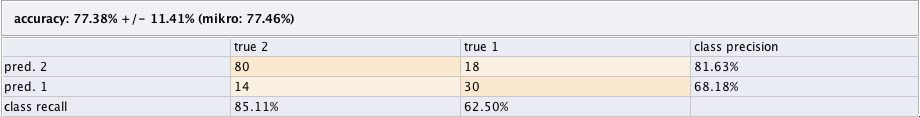
\includegraphics[width=16.09cm]{frustration-accuracy.png}} \caption{Precisión
    del modelo de clasificación para el estado mental de frustración.
} \label{frustration-accuracy}
\end{figure}

\begin{figure}[htp]
  \centerline{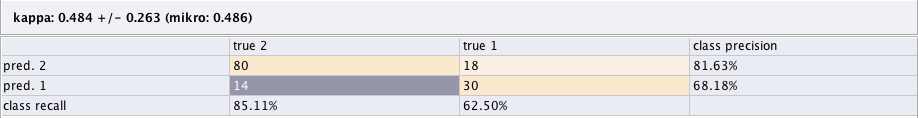
\includegraphics[width=16.09cm]{frustration-kappa.png}} \caption{Coeficiente
    de kappa del modelo de clasificación para el estado mental de frustración.
} \label{frustration-kappa}
\end{figure}


% boredom
\begin{figure}[htp]
  \centerline{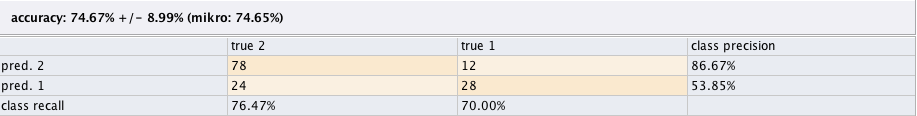
\includegraphics[width=16.09cm]{boredom-accuracy.png}} \caption{Precisión
    del modelo de clasificación para el estado mental de aburrimiento.
} \label{frustration-accuracy}
\end{figure}

\begin{figure}[htp]
  \centerline{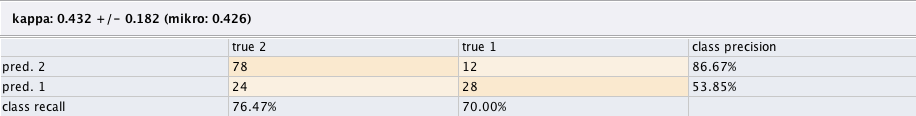
\includegraphics[width=16.09cm]{boredom-kappa.png}} \caption{Coeficiente
    de kappa del modelo de clasificación para el estado mental de aburrimiento.
} \label{frustration-kappa}
\end{figure}
%% This is an example first chapter.  You should put chapter/appendix that you
%% write into a separate file, and add a line \include{yourfilename} to
%% main.tex, where `yourfilename.tex' is the name of the chapter/appendix file.
%% You can process specific files by typing their names in at the 
%% \files=
%% prompt when you run the file main.tex through LaTeX.

\chapter{Conclusiones y Trabajo Futuro}


\section{Conclusiones}


\section{Trabajo Futuro}


\appendix
\chapter{Tables}

%\begin{table}
%\caption{Armadillos}
% \label{arm:table}
% \begin{center}
% \begin{tabular}{||l|l||}\hline
% Armadillos & are \\\hline
% our	   & friends \\\hline
% \end{tabular}
% \end{center}
% \end{table}

\clearpage
\newpage

\chapter{Figures}

\vspace*{-3in}

% \begin{figure}
% \vspace{2.4in}
% \caption{Armadillo slaying lawyer.}
% \label{arm:fig1}
% \end{figure}
% \clearpage
% \newpage

% \begin{figure}
% \vspace{2.4in}
% \caption{Armadillo eradicating national debt.}
% \label{arm:fig2}
% \end{figure}
\clearpage
\newpage

%% This defines the bibliography file (main.bib) and the bibliography style.
%% If you want to create a bibliography file by hand, change the contents of
%% this file to a `thebibliography' environment.  For more information 
%% see section 4.3 of the LaTeX manual.
\begin{singlespace}
\bibliography{main}
\bibliographystyle{plain}
\end{singlespace}

\end{document}

